\documentclass{article}
\usepackage[utf8]{inputenc}
\usepackage[top=1in, bottom=1.2in, left=0.73in, right=0.73in]{geometry}
\usepackage{hyperref}
\usepackage{graphicx}
\usepackage{datatool, filecontents}
\DTLsetseparator{,}

% Loading Data from texData.dat file
\DTLloaddb[noheader, keys={thekey,thevalue}]{texData}{../scripts/texData.dat}
\newcommand{\var}[1]{\DTLfetch{texData}{thekey}{#1}{thevalue}}

\graphicspath{ {../plots/} }
\hypersetup{
    colorlinks=true,
    linkcolor=blue,
    filecolor=magenta,
    urlcolor=cyan,
}

\title{Auto-generated Report on ICC Men's Ranking}
\author{Author: Python Program}
\date{Dated: \var{day}-\var{month}-\var{year}}

\renewcommand{\contentsname}{\LARGE{Table Of Contents}}

\begin{document}
    \maketitle

    \vspace{1cm}

    \tableofcontents

    \newpage
    % T20i Format Section
    \section{T20i Format}\label{sec:t20i-format}
        % Batting Subsection
        \subsection{Batting}\label{subsec:batting1}
            \hspace{10mm} \textbf{Rank 1 Player:}\\
            \null\hspace{10mm} Name: \var{t20i-batting-name}\\
            \null\hspace{10mm} Team: \var{t20i-batting-team}\\
            \null\hspace{10mm} Rating: \var{t20i-batting-rating}\\
            \null\hspace{10mm} Best Rating: \var{t20i-batting-best-rating}
            \vspace{1em}\\
            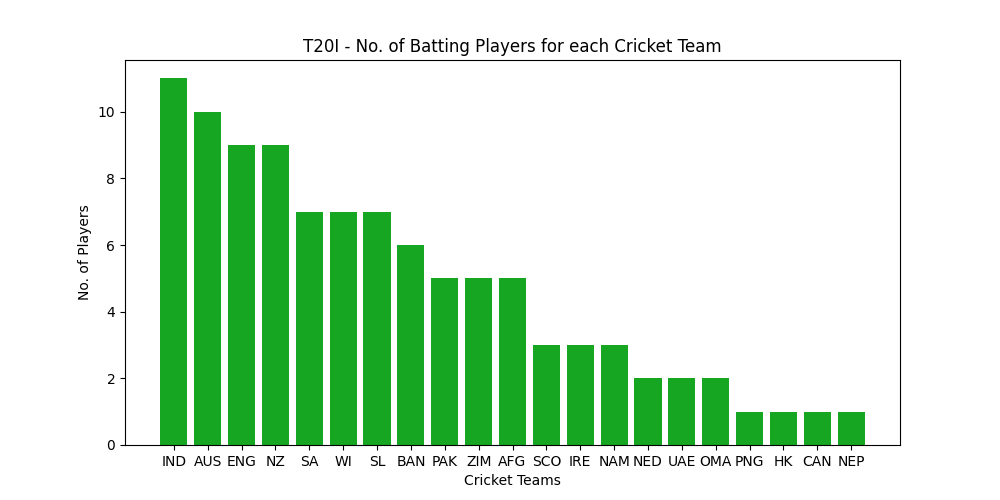
\includegraphics[scale=0.7]{t20i_batting_total_players}
            \vspace{1em}\\
            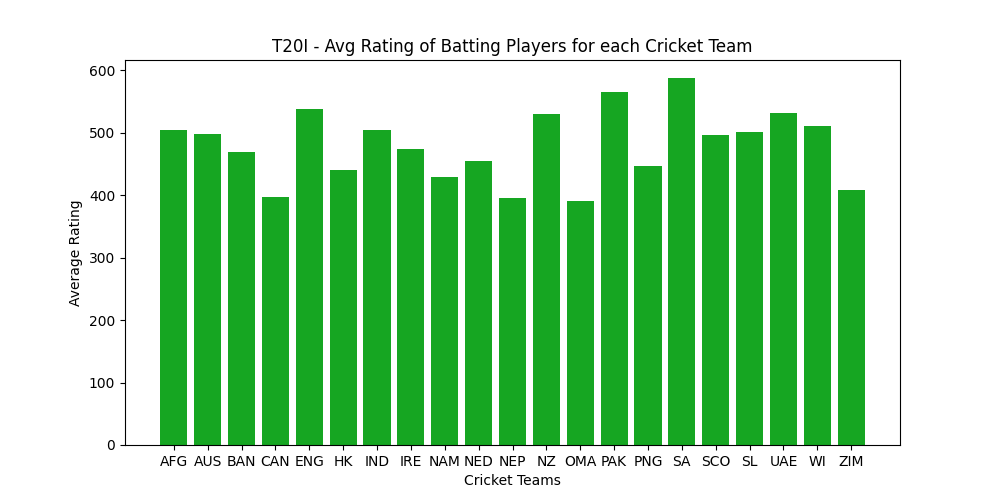
\includegraphics[scale=0.7]{t20i_batting_avg_rating}

        \newpage

        % Bowling Subsection
        \subsection{Bowling}\label{subsec:bowling1}
            \hspace{10mm} \textbf{Rank 1 Player:}\\
            \null\hspace{10mm} Name: \var{t20i-bowling-name}\\
            \null\hspace{10mm} Team: \var{t20i-bowling-team}\\
            \null\hspace{10mm} Rating: \var{t20i-bowling-rating}\\
            \null\hspace{10mm} Best Rating: \var{t20i-bowling-best-rating}
            \vspace{1em}\\
            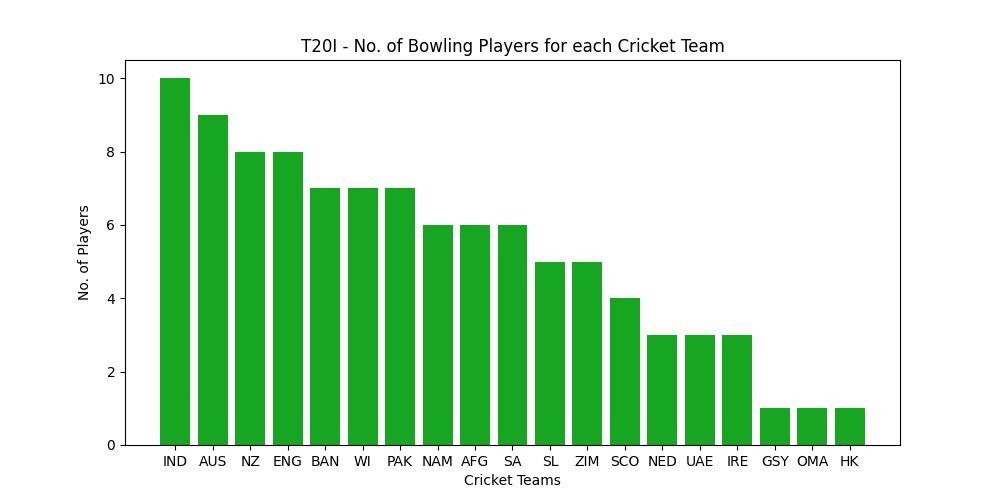
\includegraphics[scale=0.7]{t20i_bowling_total_players}
            \vspace{1em}\\
            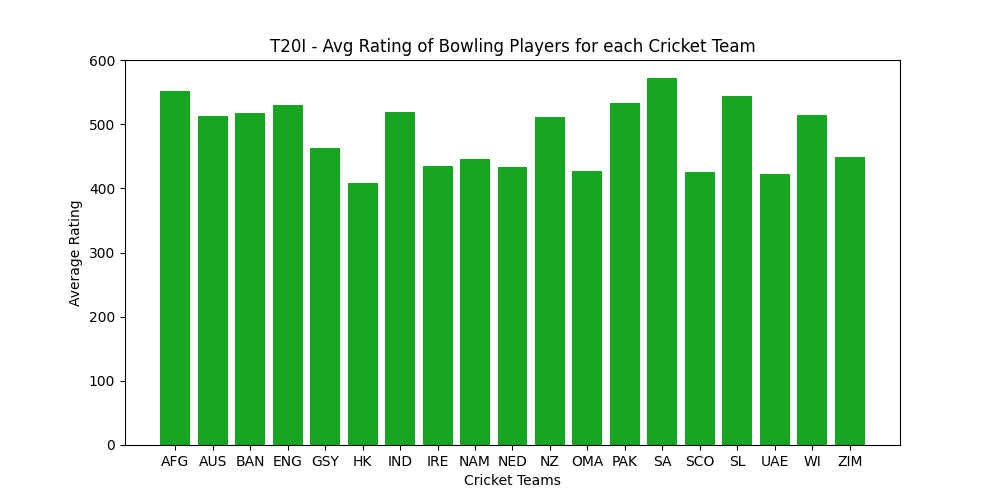
\includegraphics[scale=0.7]{t20i_bowling_avg_rating}

        \newpage

        % All-Rounder Subsection
        \subsection{All-Rounder}\label{subsec:all-rounder1}
            \hspace{10mm} \textbf{Rank 1 Player:}\\
            \null\hspace{10mm} Name: \var{t20i-all-rounder-name}\\
            \null\hspace{10mm} Team: \var{t20i-all-rounder-team}\\
            \null\hspace{10mm} Rating: \var{t20i-all-rounder-rating}\\
            \null\hspace{10mm} Best Rating: \var{t20i-all-rounder-best-rating}
            \vspace{1em}\\
            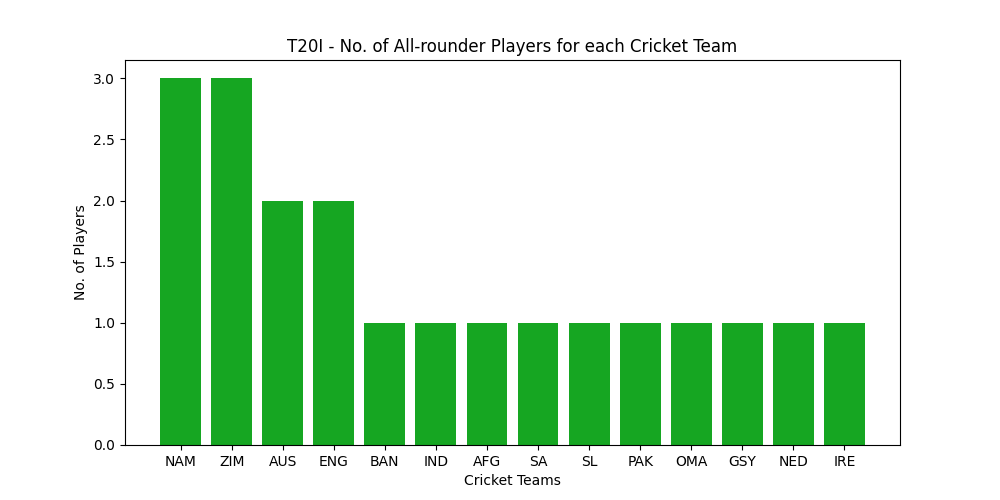
\includegraphics[scale=0.7]{t20i_all-rounder_total_players}
            \vspace{1em}\\
            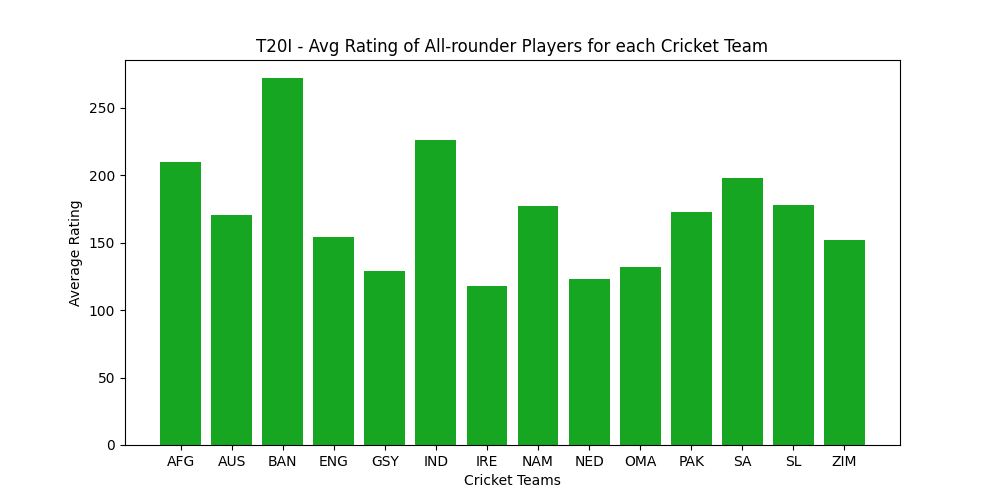
\includegraphics[scale=0.7]{t20i_all-rounder_avg_rating}

    \newpage

    % ODI Format Section
    \section{ODI Format}\label{sec:odi-format}
        % Batting Subsection
        \subsection{Batting}\label{subsec:batting2}
            \hspace{10mm} \textbf{Rank 1 Player:}\\
            \null\hspace{10mm} Name: \var{odi-batting-name}\\
            \null\hspace{10mm} Team: \var{odi-batting-team}\\
            \null\hspace{10mm} Rating: \var{odi-batting-rating}\\
            \null\hspace{10mm} Best Rating: \var{odi-batting-best-rating}
            \vspace{1em}\\
            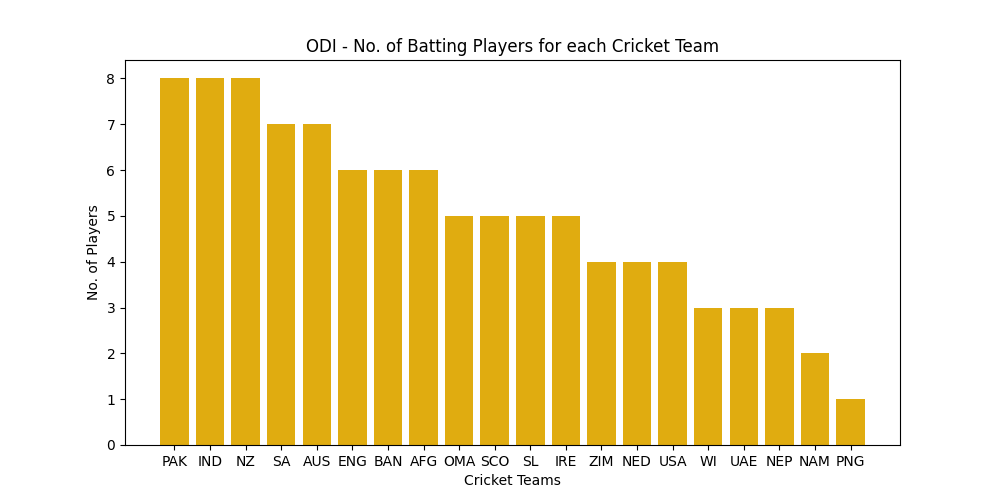
\includegraphics[scale=0.7]{odi_batting_total_players}
            \vspace{1em}\\
            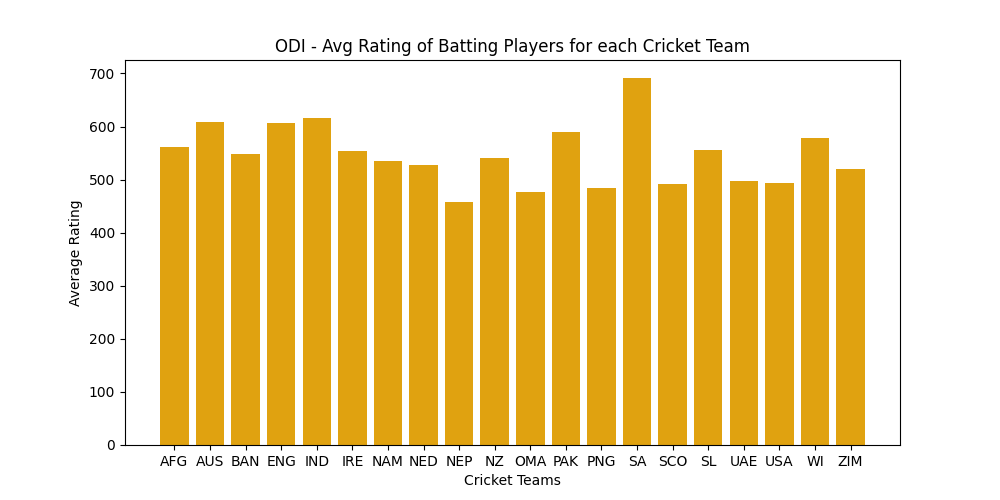
\includegraphics[scale=0.7]{odi_batting_avg_rating}

        \newpage

        % Bowling Subsection
        \subsection{Bowling}\label{subsec:bowling2}
            \hspace{10mm} \textbf{Rank 1 Player:}\\
            \null\hspace{10mm} Name: \var{odi-bowling-name}\\
            \null\hspace{10mm} Team: \var{odi-bowling-team}\\
            \null\hspace{10mm} Rating: \var{odi-bowling-rating}\\
            \null\hspace{10mm} Best Rating: \var{odi-bowling-best-rating}
            \vspace{1em}\\
            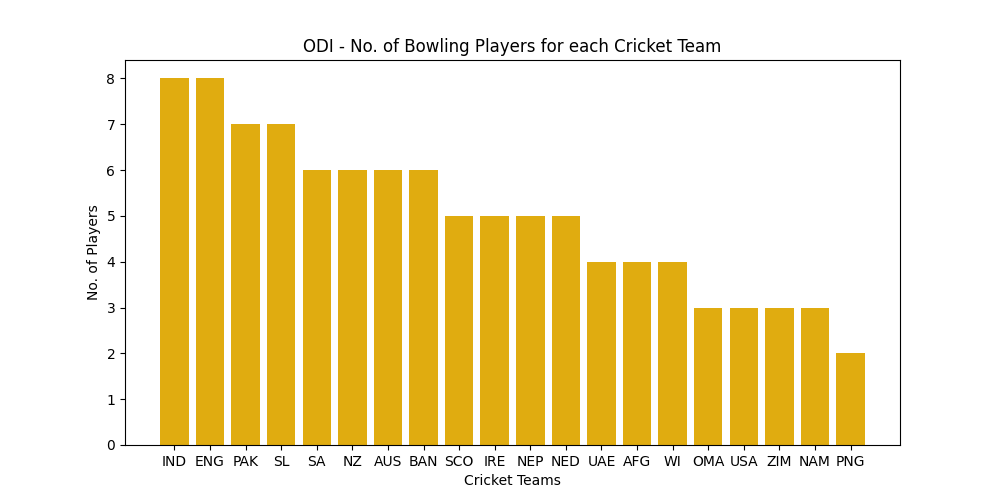
\includegraphics[scale=0.7]{odi_bowling_total_players}
            \vspace{1em}\\
            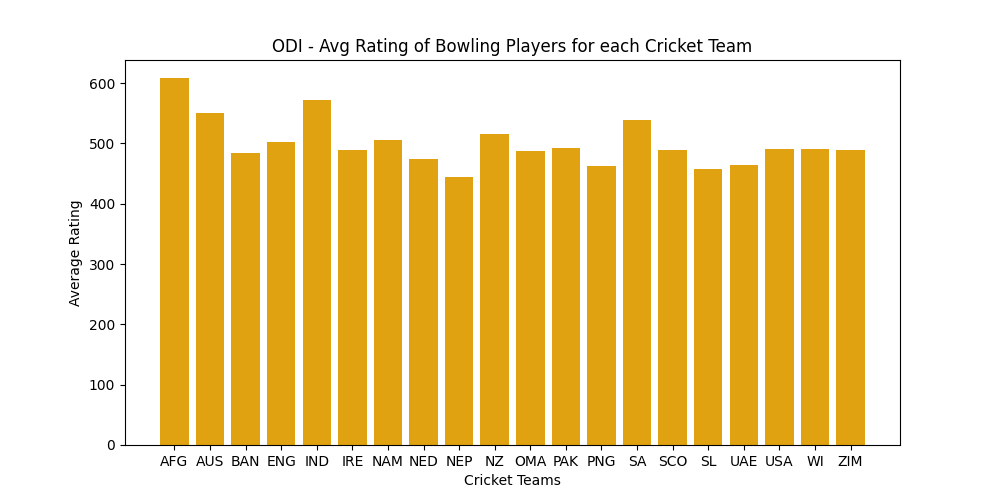
\includegraphics[scale=0.7]{odi_bowling_avg_rating}

        \newpage

        % All-Rounder Subsection
        \subsection{All-Rounder}\label{subsec:all-rounder2}
            \hspace{10mm} \textbf{Rank 1 Player:}\\
            \null\hspace{10mm} Name: \var{odi-all-rounder-name}\\
            \null\hspace{10mm} Team: \var{odi-all-rounder-team}\\
            \null\hspace{10mm} Rating: \var{odi-all-rounder-rating}\\
            \null\hspace{10mm} Best Rating: \var{odi-all-rounder-best-rating}
            \vspace{1em}\\
            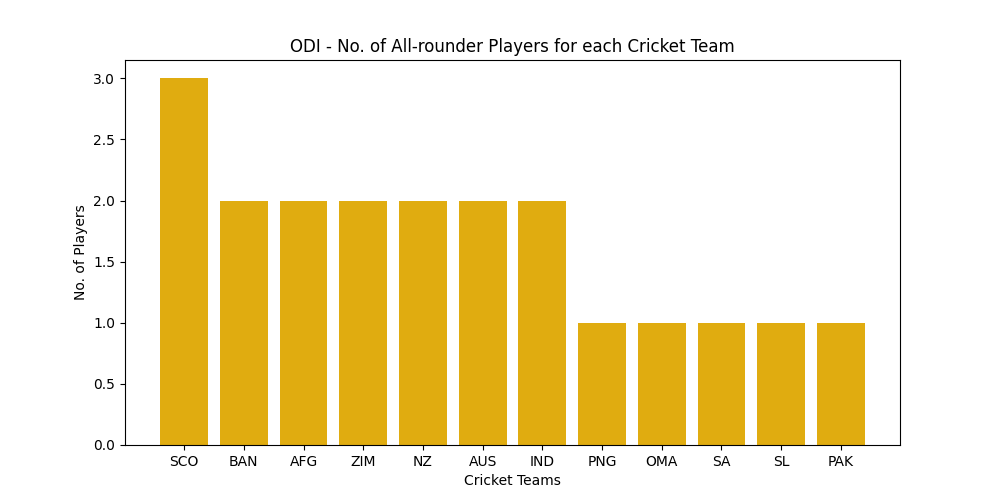
\includegraphics[scale=0.7]{odi_all-rounder_total_players}
            \vspace{1em}\\
            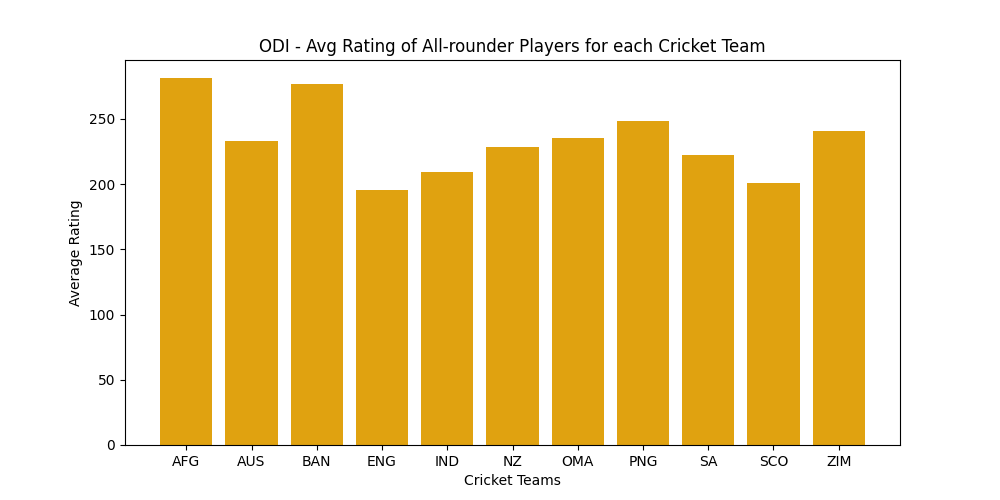
\includegraphics[scale=0.7]{odi_all-rounder_avg_rating}

    \newpage

    % Test Format Section
    \section{Test Format}\label{sec:test-format}
        % Batting Subsection
        \subsection{Batting}\label{subsec:batting3}
            \hspace{10mm} \textbf{Rank 1 Player:}\\
            \null\hspace{10mm} Name: \var{test-batting-name}\\
            \null\hspace{10mm} Team: \var{test-batting-team}\\
            \null\hspace{10mm} Rating: \var{test-batting-rating}\\
            \null\hspace{10mm} Best Rating: \var{test-batting-best-rating}
            \vspace{1em}\\
            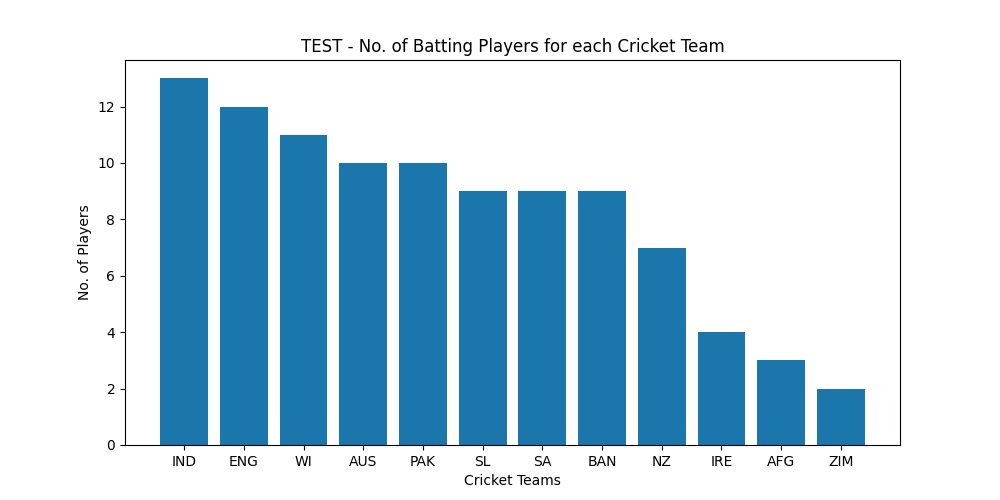
\includegraphics[scale=0.7]{test_batting_total_players}
            \vspace{1em}\\
            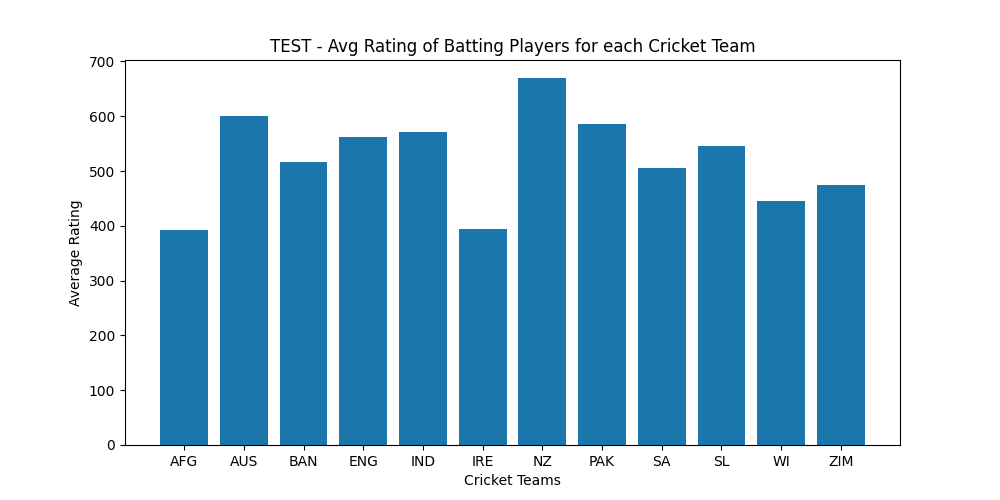
\includegraphics[scale=0.7]{test_batting_avg_rating}

        \newpage

        % Bowling Subsection
        \subsection{Bowling}\label{subsec:bowling3}
            \hspace{10mm} \textbf{Rank 1 Player:}\\
            \null\hspace{10mm} Name: \var{test-bowling-name}\\
            \null\hspace{10mm} Team: \var{test-bowling-team}\\
            \null\hspace{10mm} Rating: \var{test-bowling-rating}\\
            \null\hspace{10mm} Best Rating: \var{test-bowling-best-rating}
            \vspace{1em}\\
            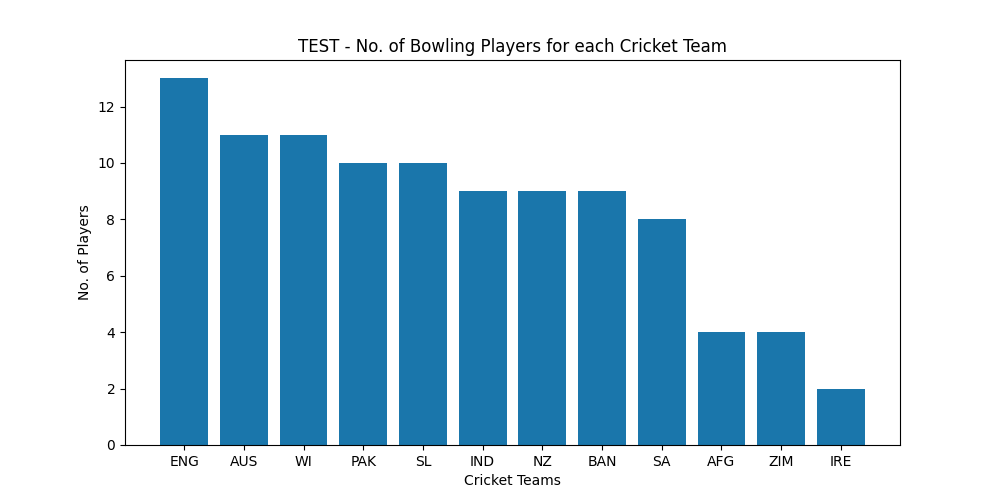
\includegraphics[scale=0.7]{test_bowling_total_players}
            \vspace{1em}\\
            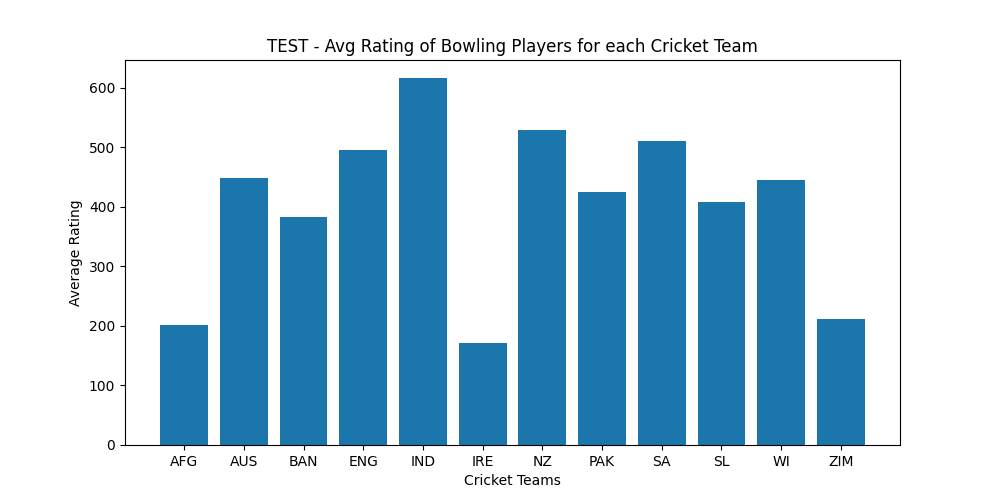
\includegraphics[scale=0.7]{test_bowling_avg_rating}

        \newpage

        % All-Rounder Subsection
        \subsection{All-Rounder}\label{subsec:all-rounder3}
            \hspace{10mm} \textbf{Rank 1 Player:}\\
            \null\hspace{10mm} Name: \var{test-all-rounder-name}\\
            \null\hspace{10mm} Team: \var{test-all-rounder-team}\\
            \null\hspace{10mm} Rating: \var{test-all-rounder-rating}\\
            \null\hspace{10mm} Best Rating: \var{test-all-rounder-best-rating}
            \vspace{1em}\\
            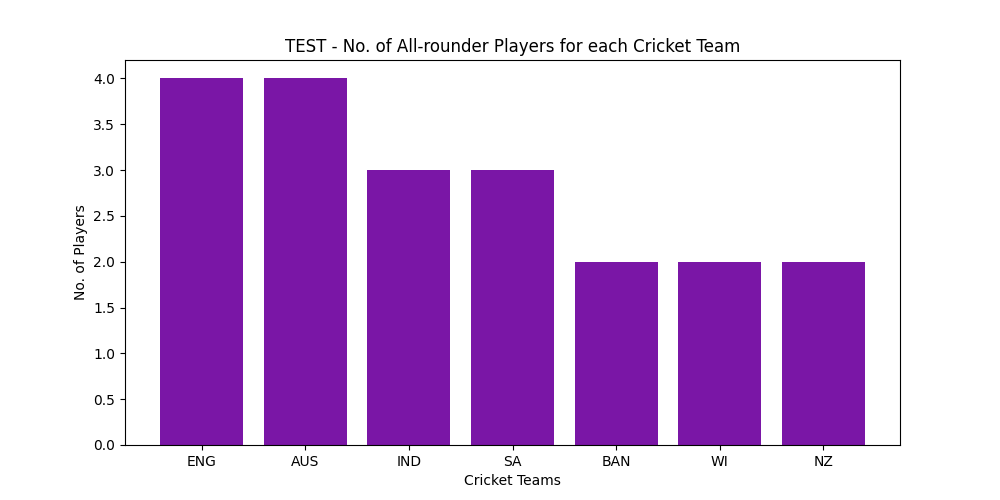
\includegraphics[scale=0.7]{test_all-rounder_total_players}
            \vspace{1em}\\
            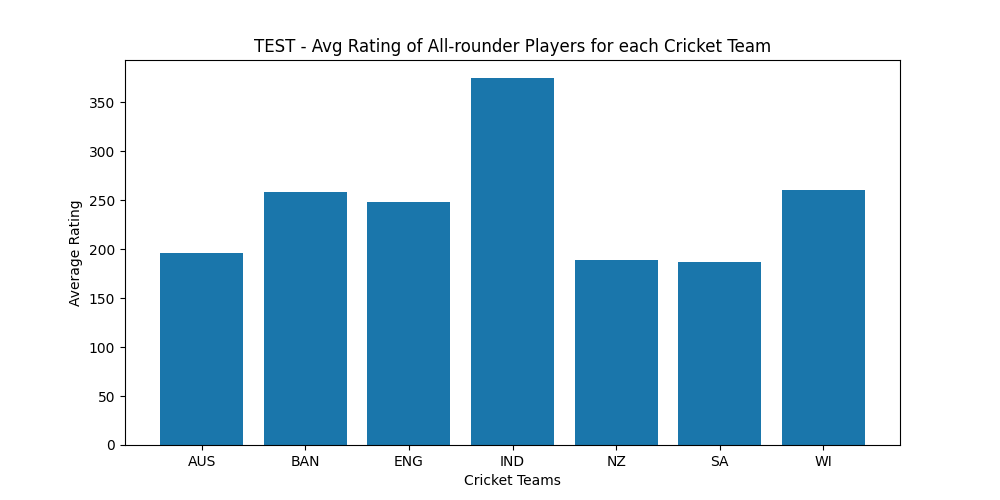
\includegraphics[scale=0.7]{test_all-rounder_avg_rating}

    \newpage

    % Overall Section
    \section{Overall}\label{sec:overall}
        % T20i Format Subsection
        \subsection{T20i Format}\label{subsec:t20i}
            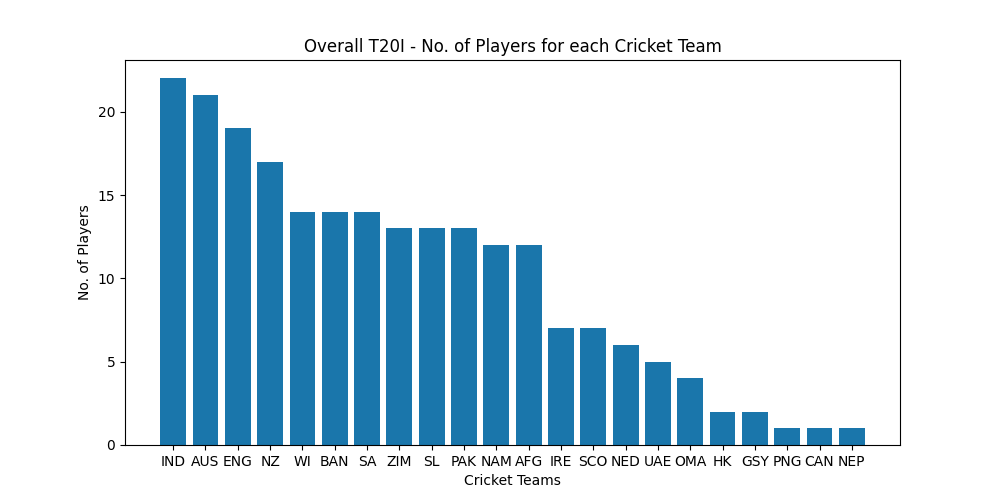
\includegraphics[scale=0.7]{overall_t20i_total_players}
            \vspace{1em}\\
            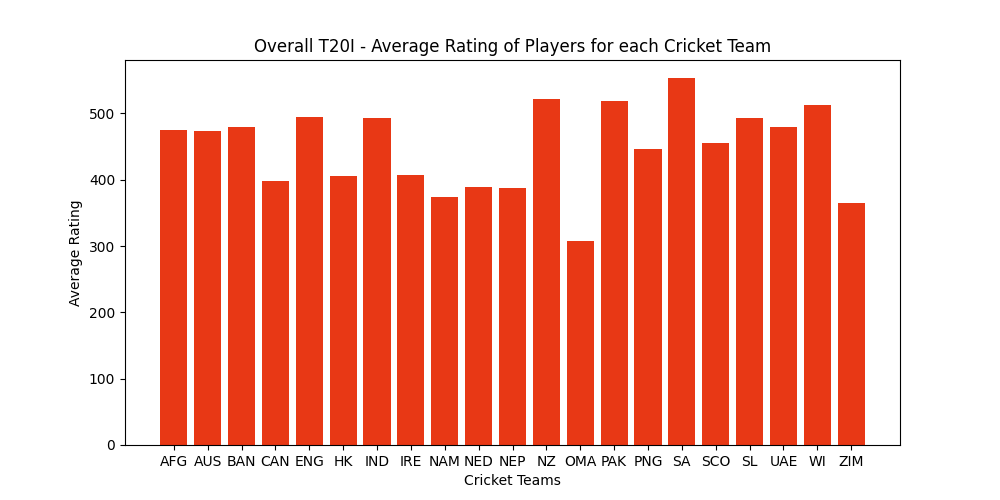
\includegraphics[scale=0.7]{overall_t20i_avg_rating}

        \newpage

        % ODI Format Subsection
        \subsection{ODI Format}\label{subsec:odi}
            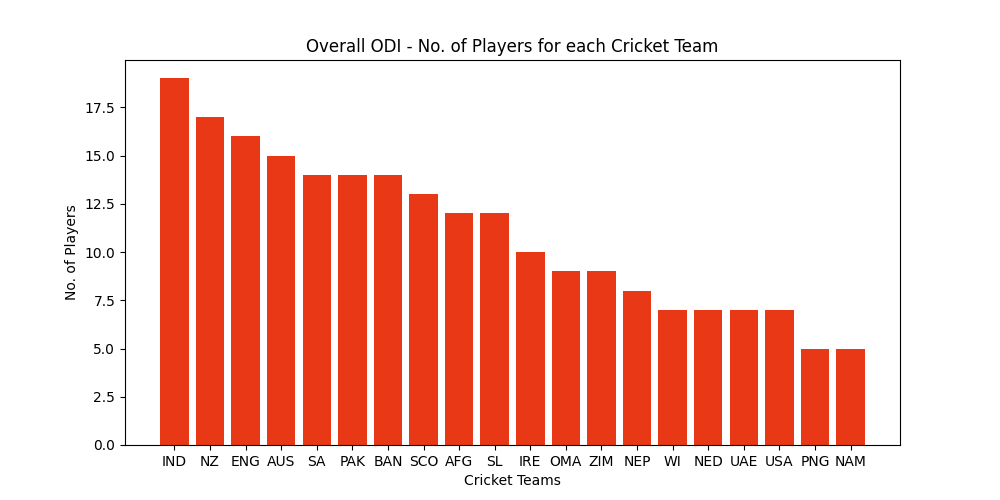
\includegraphics[scale=0.7]{overall_odi_total_players}
            \vspace{1em}\\
            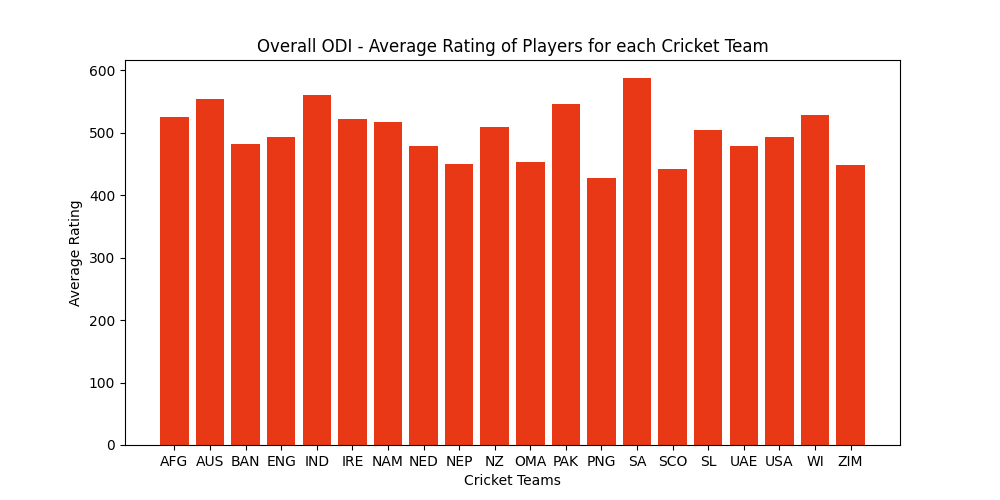
\includegraphics[scale=0.7]{overall_odi_avg_rating}

        \newpage

        % Test Format Subsection
        \subsection{Test Format}\label{subsec:test}
            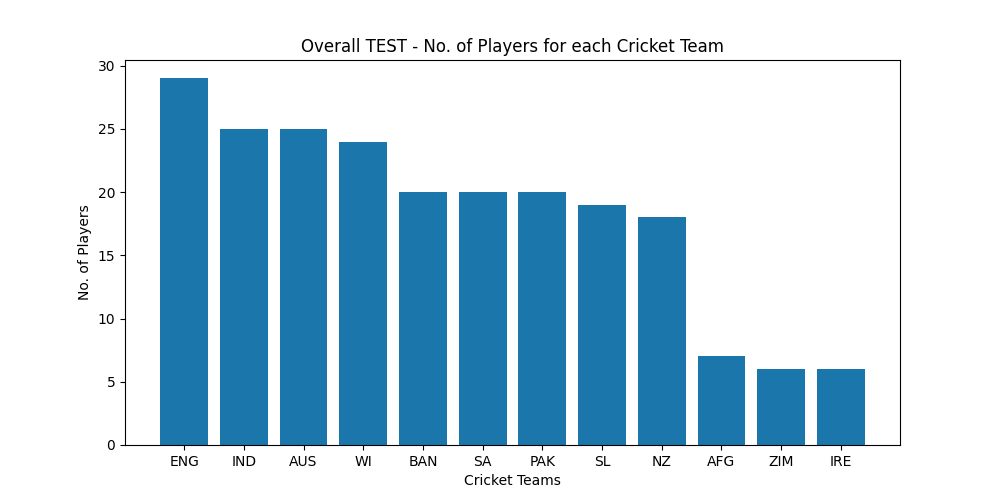
\includegraphics[scale=0.7]{overall_test_total_players}
            \vspace{1em}\\
            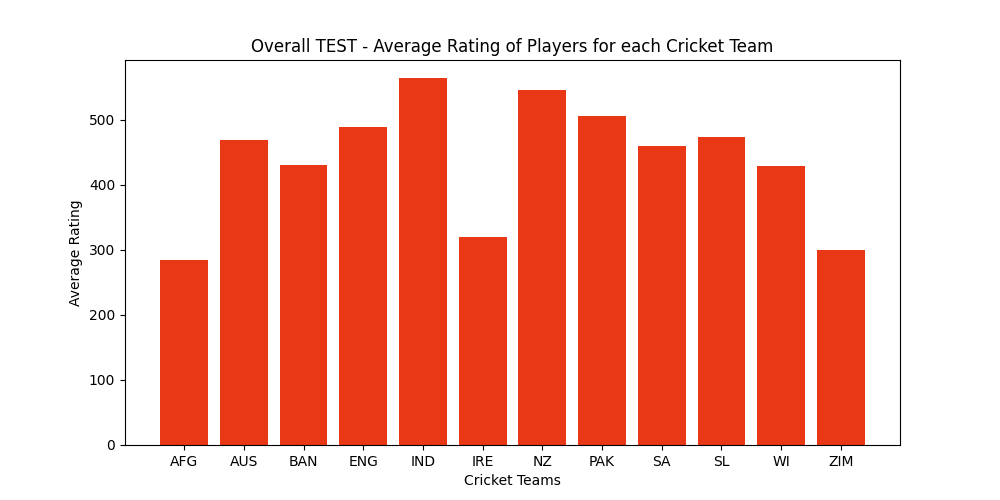
\includegraphics[scale=0.7]{overall_test_avg_rating}

\end{document}
